\documentclass{article}[10pt]

\usepackage{fullpage}

\usepackage[english]{babel}
\usepackage{graphicx}

\title{Scientific Visualization and Virtual Reality – Exercise 1}
\author{Maarten Inja (5872464) \& Chiel Kooijman (5743028)}

\begin{document}
\maketitle

We have been given a data file data lists attributes of 392 cars. The
attributes, with the data types classified by us (assignment 1), and the visual
attribute we chose to represent that data type in the visualization (assignment
2) is given in table \ref{tab:mainTable}.

\begin{table}
    \begin{tabular}{l l | l l}
    \textbf{Attribute} & \textbf{Data Type} & \textbf{Data Class} & \textbf{Visual Attribute}\\
    \hline
    \textit{model} & string & Nominal       &  Value \\
    \textit{MPG} & num & Quantative Ratio   & Shape/Angle/Value \\
    \textit{cylinders} & num & Quantitive Ratio & Color \\
    \textit{horsepower} & num & Quantative Ratio & Position\\
    \textit{weight (lbs)} & num & Quantative Ratio & Area \\
    \textit{year} & num & Quantative Interval & Position \\
    \textit{origin} & string & Nominal & Position
    \end{tabular}
\caption{The main table showing the data class determined by us, and our chosen
visual attribute}
\label{tab:mainTable}
\end{table}

\section{Data Class}
One could argue that the amount of cylinders is
nominal since there is a fixed number of options (3, 4, 5, 6, 7 and 8). However,
we have selected Quantitative Ratio because there is fixed 0, and a ratio can be
calculated.

\section{Bertin's Visual Attributes}

We plot each car in a graph.
In these graphs the year will be on the x-axis, because that seems intuitive as the time
is often placed on the x-axis. On the y-axis we will show the horsepower, so
higher means more horsepower.
Together these two properties will determine the position of a data point.
Since there only three points of origin we can divide the y axis of the graph
in three of the same graphs with the different data for each point of origin. In
this way the x-axis (time) is shared for all cars independent of their origin.

The data point will be represented by a polygon in which the amount of
vertices/corners indicates the amount of cylinders (i.e. triangle = 3 cylinders,
square = 4 cylinders), in this way we lose no information. The size of the
polygon indicates the weight of the car.
Next to the data point we can print the model name.
Finally, the greyness of the polygon determines the miles per gallon. Black
indicates inefficient cars and white efficient cars. This could be changed to
color but we feel that black is better because in our culture black has a
negative association and because the soot, polluting exhaust gasses
(of those inefficient cars) might be blacker as well.

We have decided on the visual attributes in such a way that more important
properties have received a more accurate attribute. Of course the importance of
certain properties is debatable. For example one could easily argue that
miles per gallon is more important that horsepower, in which case the attributes
should be swapped.

Since there are many model names they might not all fit. An interactive version
of the graph would solve this problem. In this case the model name should be
displayed if the users hovers over the data entry. An non-interactive
alternative would a look up table: supply the graph with a look up table and
print the row number of the model name next to each polygon.

\section{Visualization}
In figure \ref{fig:vis} is our visualization. We used Python with Matplotlib to
create this visualization. Unfortunately there was no room to write the model in
the graph.

\begin{figure}[h!]
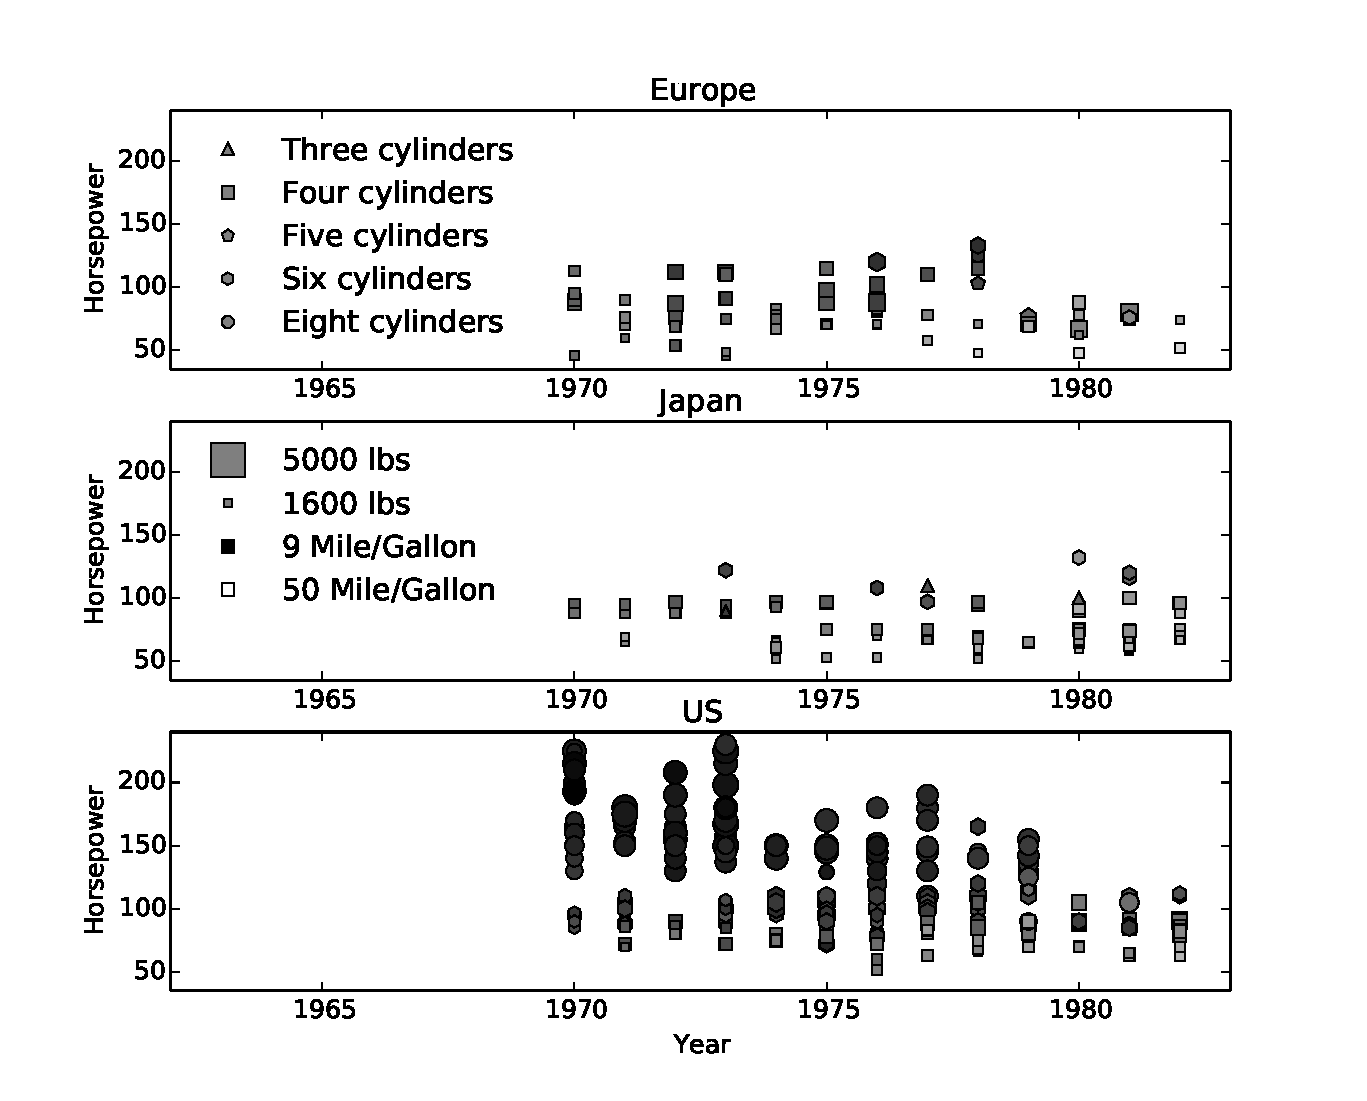
\includegraphics[width=\textwidth]{autovis}
\caption{The visualization of cars for three regions.}
\label{fig:vis}
\end{figure}

We feel that this visualization is effective as it quickly shows certain trends
in the development of the cars over time (overall, cars became less heavy and more
efficient)
and the difference of cars from different regions (American cars are in general
heavier and less efficient but have more horsepower). This visualization does
not work well for comparing different car models. However, we feel that his is
not a big problem because a look up table is inherently better for such a purpose.


\end{document}
